Placile video se ocupa in marea partea a timpului cu randarea imaginii care se afiseaza pe ecran.
Acest lucru presupune generarea unei imagini care contine foarte multi pixeli la un refresh rate de
aproximativ 60 de cadre pe secunda. 

Doar pentru a genera 60 de cadre pe secunda, este nevoie de un bus capabil sa trimita date cu o
viteza de minim 4GBit/s.

Fiecare cadru este compus din aproximativ 2 milioane de pixeli. Aceasta viteza este atinsa datorita
faptului ca fiecare pixel este calculat individual, placile video fiind un exemplu ideal de
procesare paralela. Incepand cu api-ul DirectX10, sau arhitectura G80 , placile video au incorporat Vertex Shader si
Pixel Shader intr-o singura unitate numita Cuda Core \cite{luebke2008gpu}. Astfel toate operatiile
de tip Vertex Shader sau Pixel shader sunt realizate de aceasi unitate Cuda Core. Acest lucru
elimita cazul in care  daca se executau operatii de tip vertex, doar Vertex Shaderul sa fie
operational si Pixel Shaderul sa fie idle, si invers.

\begin{figure*}[ht] \centering
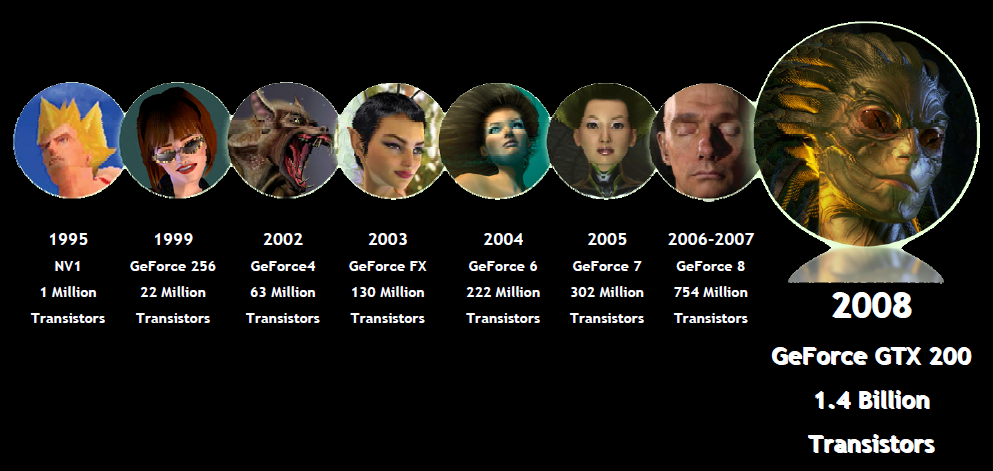
\includegraphics[width=0.9\textwidth]{img/evolution.png}
\caption{Evolutia placilor video 3D} \end{figure*}

\subsection{Cuda Core}

Spre deosebire de un procesor clasic, care se bazeaza pe un numar mic de nuclee, intre 1 si 16, un
procesor grafic foloseste un numar mult mare, de exemplu 3072 de Cuda Cores, in cazul placi Nvidia Geforce
Titan X \cite{titanx}, dar si de o latime de banda net superioara unui procesor clasic, o latime de 336.5 GB/s.

Fiecare Cuda Core se aseamana ca functionalitate in mare parte cu un nucleu al unui procesor
normal, dar acesta ruleaza la o frecventa mult mai mica, de aproximativ 3-4 ori mai mica, si au
functionalitati limitate, pentru a mentine suprafata fizica a acestuia cat mai mica.

Deoarece numarul nucleelor Cuda este atat de mare, multihreading-ul este implementat hardware,
pentru a reduce cat mai mult overhead-ul datorat de planificarea threadurilor. Pentru a simplica
aceasta planificare, nucleele sunt grupate in clustere, fiecare cluster executand aceeasi
intructiunie. Acest lucru este posibil deoarece procesoarele video se bazeaza pe o arhitectura de tip SIMT - Single Instruction Multiple Threads \cite{luebke2008gpu}.

\begin{figure*}[ht] \centering
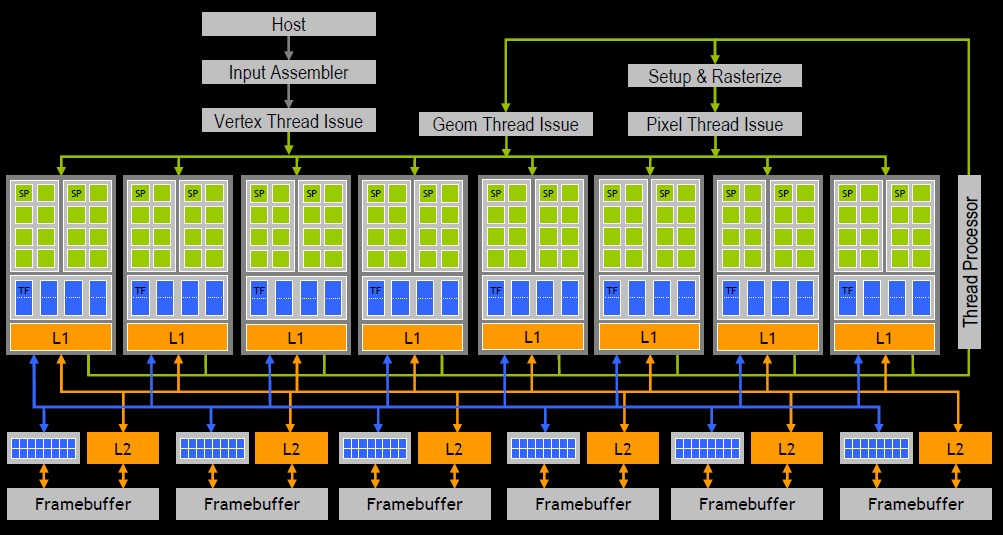
\includegraphics[width=0.9\textwidth]{img/g80.png}
\caption{Arhitectura Nvidia G80} \end{figure*}


\subsection{Arhitectura Fermi - 2010}

Arhitectura Fermi a continuat arhitectura G80, astfel ca fiecare Cluster de Cuda Core, sau Procesoarea Stream,
contin 32 de procesoare Cuda. Acestea au ramas la fel de complexe ca cele anterioare dar
numarul lor a crescut la 512.

\subsection{Arhirectura Kepler - 2012}

In arhitectura Kepler, numarul de Procesoare Stream a scazut de la 16 la 8, astfel fiecare cluster
continea 192 de procesoare Cuda. Pe langa numarul crescut de procesoare Cuda, acesteau au fost
simplicate, pentru a obtine o viteza de executie mai mare dar si un consum mai redus. In
arhitectura Fermi, procesoarele Cuda functionau la o frecventa dubla fata de cea a GPU-ului, dar in
acesta arhitectura, deoarece functioneaza la o frecventa mult mai redusa, consumul lor este cu 90\%
mai mic decat cele ale arhitecturii precedente. Acest lucru a permis triplarea procesoarelor Cuda de la 512 la 1536.

\subsection{Arhitectura Maxwell - 2014}

Ducand mai departe ideea de performanta marita pentru un consum redus, arhitectura Maxwell a
eficientizat arhitectura Kepler, astfel ca 128 de Cuda Cores Maxwell sunt la fel de rapide ca 192
de Cuda Cores de tip Kepler. Deasemenea a implementat un algoritm de compresie a texturilor, ceea
ce a permis pastrarea aceleiasi latimi de banda a memoriei cu o creste a performantei.

